% Chapter Template

\chapter{Introduction} % Main chapter title

\label{Chapter1} % Change X to a consecutive number; for referencing this chapter elsewhere, use \ref{ChapterX}

%----------------------------------------------------------------------------------------
%	SECTION 1
%----------------------------------------------------------------------------------------
Taking a photograph of an object, traditionally, we need to face a camara (detector) to the object. But with two-photon imaging 
we use a detector that is towards the light source, rather than towards the object.
As the name suggest it, we also use the information about another photon that is strongly correlated. (IMAGE)
 Two-photon is reproduced at quantum level by a non-factorizable point-to-point image-forming correlation between two photons.

Two-photon imaging has been demonstrated using two types of light sources. Type-one
two-photon imaging uses entangled photon pairs as the light source. In 1995 Pittman, realized a 
quantum two-photon geometric optical effect.  They have successfully performed optical 
imaging by means of a quantum-mechanical entangled source\cite{pittman}.

Type-two of imaging uses chaotic light. The type-two  
image-forming correlation is caused by the superposition between paired two-photon amplitudes,
or the symmetrized effective two-photon wave-function\cite{physicsGhost}.
\section{Imaging}

Assuming we have an object that have its own light or its externally illuminated,
imaging means collecting that light that is emitted from the object. Each point
of the surface od the object will emit spherical waves to all possible directions,
been this said, What is the probability to have a spherical wave collapsing into a point or small spot? 
Obviously, the chance is practically zero unless an imaging system is applied.
\\
The concept of optical imaging was well developed in classical optics and the Figure
\ref{fig:imaging} schematically illustrates a standar imaging setup. In this setup 
an object is illuminated by a radiation source, an imaging lens is used 
to focus the scattered and reflected light from the object onto an image plane 
which is defined by the “Gaussian thin lens equation”\cite{hecht}:
\begin{equation}
\frac{1}{s_0}+\frac{1}{s_i}=\frac{1}{f}
\end{equation}
 where $s_0$ is the distance between the object and the imaging lens, $s_i$ the distance 
between the imaging lens and the image plane, and $f$ the focal lenght of the imaging lens. This equation defines
a point-to-point relationship between the object plane and the image plane: any radiation starting from a point on the object will colapse at a certain point at the image plane.
\\
\begin{figure}[h!]
\centering
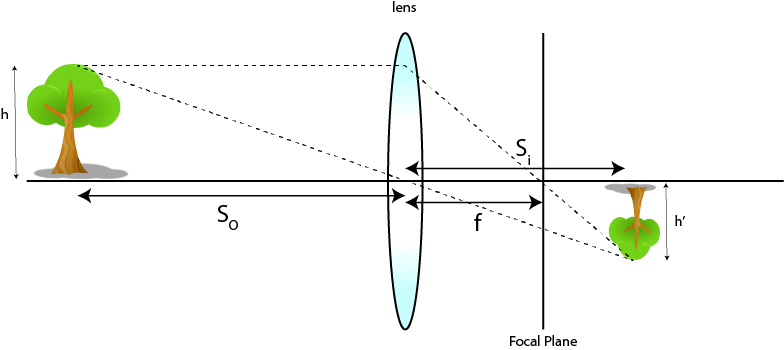
\includegraphics[width=0.6\textwidth]{Figures/imaging.png}
\caption{Optical imaging: a lens produces an image on an object at $f+d$. This distance is defined
by the Gaussian thin-lens equation $\frac{1}{l}+\frac{1}{f+d}=\frac{1}{f}$} 
\label{fig:imaging}
\end{figure}
This one-to-one correspondence in the image-forming relationship between the object and the image planes produces a perfect image.
The observed image can be magnified or demagnified, for example, in the 
Figure \ref{fig:imaging} the original object is a tree, and it is demagnified at the image plane. This depends on which optical 
system are we using, what kind on lenses are involved and the distance between object and them.
The observed image is a reproduction of the illiminated object, mathematically
corresponding to a convolution between the object distribution fuction $ |T(\vec{\rho_o})|^2$ (aperture function) and a $\delta$-function, which is present for the perfect
point-to-point correspondence\cite{introquantum}:
\begin{equation}
I(\vec{\rho_i})=\int_{obj} d\vec{\rho_o} |T(\vec{\rho_o})|^2 \delta(\vec{\rho_o}+\frac{\vec{\rho_i}}{m})
\end{equation}
where $I(\vec{\rho_i})$ is the intensity at the image plane, $\vec{\rho_o}$ and $\vec{\rho_i}$ are 2-D vectors of the
transverse coordinates in the object and image planes, respectively, and
$m=s_i/s_o$ is the image magnification factor.

In reality, we are limited by the finite size of the optical system, we may never obtain a perfect image.
we have to take into account the constructive-destructive interference present
in this phenomena, because of the wave nature of light. The point-to-point correspondence turns into a point-to-"spot" relationship.
For further informations about this "real life" situation check the \ref{app:intensity}.



%-----------------------------------
%	SUBSECTION 1
%-----------------------------------
\section{Two-Photon Imaging}

The optical imaging used the photons at the image plane to form the image, in other 
words it take measure one photon per spot at the image plane. For the type-one and type-two
two-photon imaging, in certain aspects the behaviour is similar as that of the classical.
They both exhibit a similar point-to-point imaging-forming function, except the 
two-photon image is only reproducible in the joint-detection between two independent photodetectors,
and the point-to-point imaging-forming function is in the form of second-order correlation,
\begin{equation}
R_{12}(\vec{\rho_i})=\int_{obj} d\vec{\rho_o} |T(\vec{\rho_o})|^2 G^{(2)}(\vec{\rho_o},\vec{\rho_i})
\end{equation}
where $R_{12}(\vec{\rho_i})$ is the joint-detection counting rate between photodetectors $D_1$ and $D_2$.
$G^{(2)}(\vec{\rho_o},\vec{\rho_i})$ is a nontrivial point-to-point second-order correlation
function, corresponding to the probability of observing a joint photo-detection event
at the coordinates $\vec{\rho_o}$ and $\vec{\rho_i}$. The physics behing $G^{(2)}(\vec{\rho_o},\vec{\rho_i})$
is what changes between type-one and type-two two-photon imaging.
\begin{figure}[h]
\centering
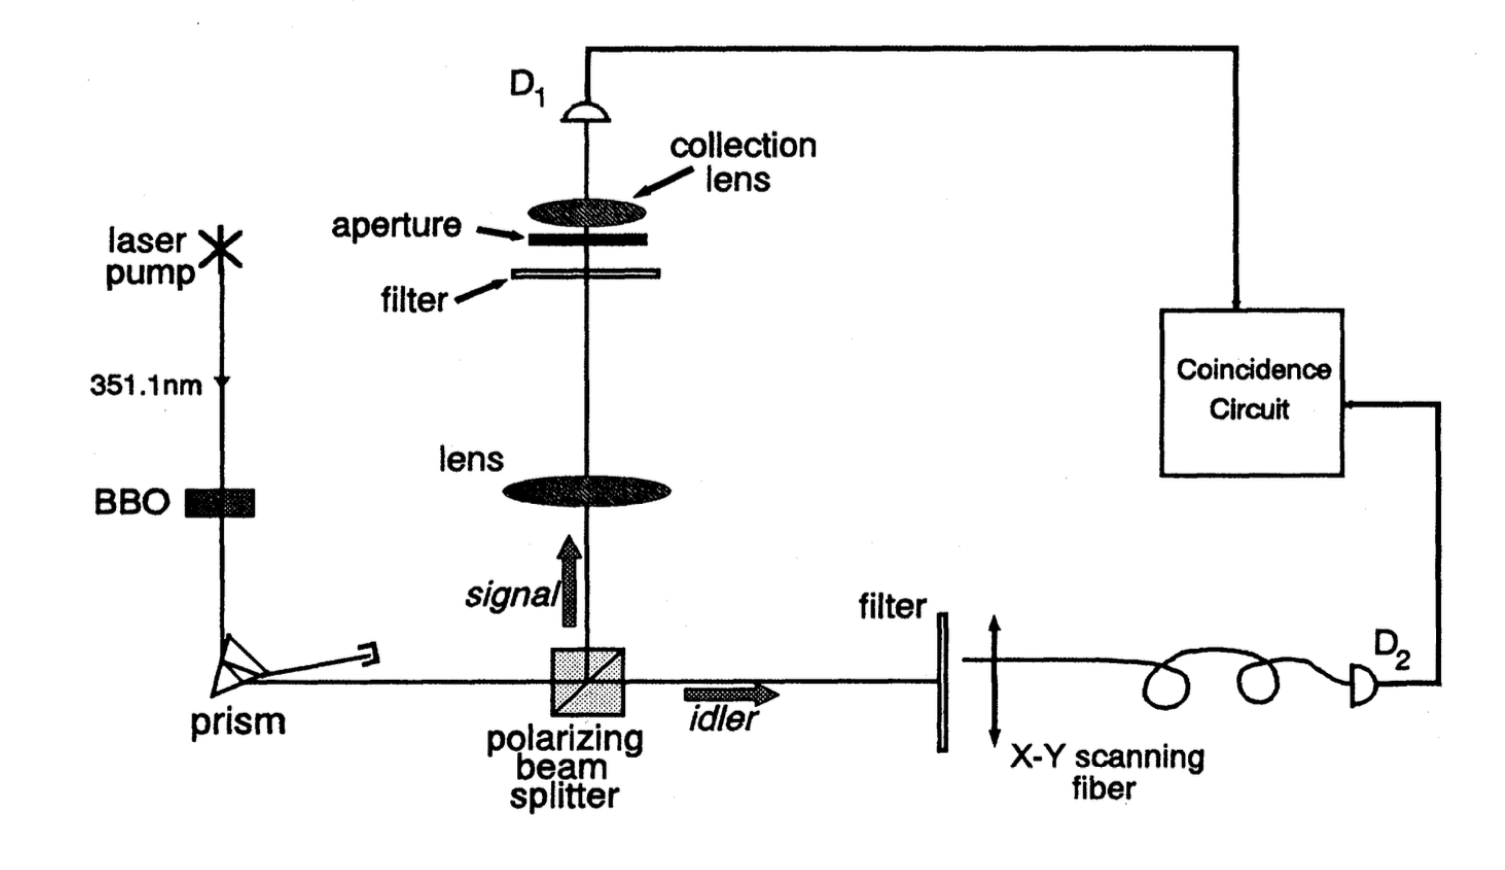
\includegraphics[width=0.5\textwidth]{Figures/pittman.png}
\caption{Schematic of the first "two-photon imaging" experimental setup, used by Pittman\cite{pittman}} 
\label{fig:pittman}
\end{figure}

\subsection{Two-Photon Imaging using entangled photon pairs}
The first type-one two-photon imaging experiment was demonstrated by Pittman
in 1995\cite{pittman}. The schematic setup of the experiment is shown in the 
Figure \ref{fig:pittman}. A continuous wave (CW) laser is used to pump a nonlinear 
crystal to produce pairs of entangled photons. 
This pairs of orthogonally polarized signal and idler photons are the product
of the nonlinear optical process of spontaneous parametric down-conversion (SPDC).
The pair emerges from the crystal collinearly, it is separated by a dispersion prism, 
and then the signal and idler are sent in different directions by a polarization
beam slitting Glan-Thompson prism. 

The experimental setup is shown in Fig. 1.A 2-mm-diam beam from the 351.1-nm 
line of an argon ion laser is used to pump a nonlinear beta barium borate (BBO)
(P-BaBz04) crystal that is cut at a degenerate type-II phase-matching angle to produce 
pairs of orthogonally polarized signal (e-ray plane of the BBO) and idler (o-ray plane 
of the BBO) photons. The pairs emerge from the crystal nearly col- linearly, 
with ~,=~;=cup/2. The pump is then separated from the slowly expanding 
down-conversion beam by a UV grade fused silica dispersion prism and the 
remaining signal and idler beams are sent in different directions by a polarization 
beam-splitting Thompson prism. The refIected signal beam passes through a 
convex lens with a 400-mm focal length and illuminates the (UMBC) aperture. 
Behind the ap- erture is the detector package $D_1$, which consists of a 25-mm 
focal length collection lens in whose focal spot is a 0.8-mm-diam dry ice 
cooled avalanche photodiode. The transmitted idler beam is met by detector 
package $D_2$, which consists of a 0.5-mm-diam multimode fiber whose output is 
mated with another dry ice cooled avalanche photodiode. Both detectors are 
preceded by 83-nm-bandwidth spectral filters centered at the degenerate 
wavelength 702.2 nm. The input tip of the fiber is scanned in the transverse 
plane by two orthogonal encoder drivers, and the output pulses of each 
detector, which are operating in the Geiger mode, are sent to a coincidence 
counting circuit with a 1.8-ns accep- tance window.


An important fact of this experiment is the use of a lens(collection lens) in the signal beam that establishes an image plane with the definitive point-by-point correspondence object(mask) plane.




\subsection{Two-photon Imaging Using Thermal Sources}

In \cite{thermal} they compared ghost Imaging using entanglement versus Classical correlated light. read and information in \cite{thermalAlejandra}. here i talk about coherence and intensity fluctuations \cite{intensity}

\subsection{Simulations}

No\cite{simulated}
%----------------------------------------------------------------------------------------
%	SECTION 2
%----------------------------------------------------------------------------------------



